\chapter{Disseny de la solució}

Per tal de complir els nostres objectius comentats en els punts anteriors, s'ha hagut de fer
un gran treball de planificació i disseny. En aquest capítol, s'intenta mostrar i justificar 
les principals decisions de disseny.

\section{Disseny general del rootkit}

L'arquitectura del rootkit és la de client-servidor. Això significa que hi ha una part que 
s'executa a una màquina que ofereix ``serveis'' (el servidor), i una part que sol·licita i
rep els serveix que ofereix l'altre. \\

A partir d'aquest moment anomenarem ``launcher'' a la part servidor del rootkit, i ``client''
a la part client. \\

En un cas típic, el launcher serà la part del rootkit que s'executarà a la màquina que haguem 
compromès, i el client serà la part que executarà l'atacant per tal de connectar-se al launcher. \\

Com a tot projecte de software, el disseny és una de les parts més importants, i per començar 
cal decidir quines característiques volem assolir. En aquest cas s'ha escollit la portabilitat, 
extensibilitat, llegibilitat i la no repetició de codi, com a característiques principals del 
nostre disseny. \\

\begin{figure}[htp]
    \centering
        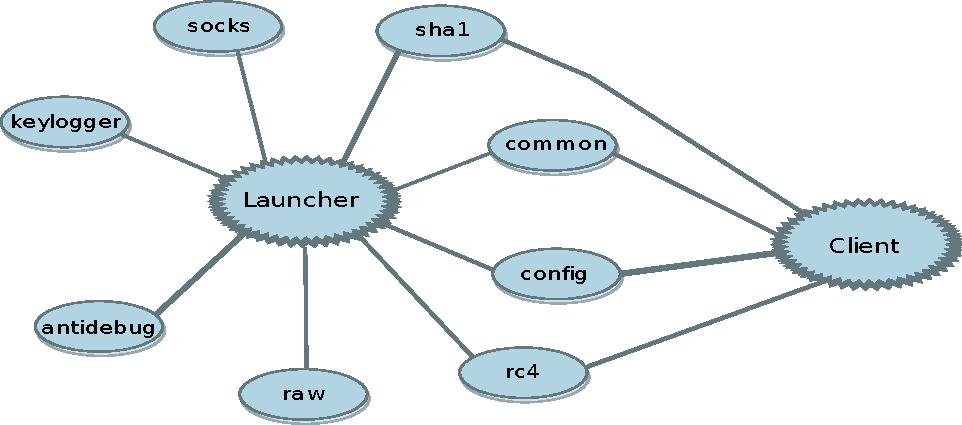
\includegraphics[scale=0.7,keepaspectratio]{diagrames/solutionDesignModules.pdf} \\
    \caption{Esquema dels diferents components que formen el rootkit}
    \label{fig:rootkitModules}
\end{figure}

\subsection{config}

En moment de compilació, el rootkit ens demana una sèrie de preguntes per tal de configurar-se a gust
de l'usuari, i per tal d'adaptar-se millor a unes característiques o a unes altres. Entre aquestes
preguntes, hi ha el password a utilitzar en la part servidora, si activar el mode debug, etc. Aquest
mòdul permet accedir a la configuració tant del launcher com del client.

\subsection{launcher}

Part nucli de la part servidor del rootkit. En aquesta part és on hi ha tota la estructura principal
de la part que s'instal·la a la màquina de la víctima.

\subsection{common}

Com el seu nom indica, és la part comuna entre mòduls, launcher i client.

\subsection{rc4}

Mòdul que ens permet xifrar la connexió utilitzant l'algoritme simètric rc4. Gràcies a aquest mòdul,
tota la informació que s'envia entre client i servidor, i client, és xifrada. 

\subsection{sha1}

Algoritme de hash utilitzat principalment per a obtenir un password d'una longitud fixa. En el moment
de compilació, el mòdul de configuració, sol·licita un password, aquest password haurà de ser especificat
per el client per tal de establir una connexió amb el launcher, i s'utilitzarà com a clau de xifratxe
de la comunicació.

\subsection{raw}

Mòdul que ens proporciona tota la funcionalitat del mode de funcionament raw. Tant la definició dels
paquets de xarxa, com les funcions dels diferents serveix necessaris.

\subsection{antidebug}

Mòdul que proveeix de les funcionalitats antidebug. Les diferents funcions que incorpora, són definides
com a inline, per tal que siguin incloses directament al codi.

\subsection{common}

Aquest mòdul incorpora les funcions genèriques més generals que utilitza el rootkit. És utilitzat tant per
el launcher, com per el client.

\subsection{keylogger}

És el mòdul que ens permet capturar passwords introduits en diferents serveis com poden ser ssh, ftp, mysql, etc.
\section{Modes de comunicació}

Tal i com hem vist en el capítol funcionalitats, aquestes varien segons els permisos que tinguem a la màquina 
i segons les nostres necessitats en cada moment. De la mateixa manera, podrem utilitzar unes tècniques per a
comunicar-nos o unes altres segons els mateixos privilegis. Aquestes tècniques són les què anomenarem modes
de comunicació, i dependran principalment dels privilegis alhora d'executar el rootkit.\\

En total tenim quatre modes de comunicació. \\

\begin{enumerate}
    \item LISTEN
    \item TCP
    \item REV
    \item RAW
\end{enumerate}

La taula de la figura  \ref{fig:tableModesRelation} ens mostra una relació dels modes de comunicació que podem utilitzar
en un entorn privilegiat i amb un entorn no privilegiat.

\begin{figure}[htp]
    \centering
    \begin{tabular}{|c|c|c|c|c|}
        \hline
         & \textbf{LISTEN} & \textbf{TCP} & \textbf{REV} & \textbf{RAW} \\ \hline
         \textbf{Entorn no privilegiat} & \textcolor{Green}{Si} & \textcolor{Green}{Si} & \textcolor{Red}{No} & \textcolor{Red}{No} \\ \hline
         \textbf{Entorn privilegiat} & \textcolor{Red}{No} & \textcolor{Red}{No} & \textcolor{Green}{Si} & \textcolor{Green}{Si} \\ \hline
    \end{tabular}
    \caption{Modes de comunicació disponibles segons el mode d'execució.}
    \label{fig:tableModesRelation}
\end{figure}

Cal dir que el fet de què en el entorn privilegiat no es puguin utilitzar els modes de comunicació LISTEN ni TCP, és degut
a que això no té sentit. Els dos modes disponibles en el mode privilegiat, són millors que els dos oferts en mode no
privilegiat. A continuació es detallen les diferencies entre aquests modes de comunicació:

\subsection{Mode no privilegiat}

Tal i com mostra la taula de la figura \ref{fig:tableModesRelation}, en un entorn no privilegiat, podem utilitzar dos modes de
comunicació. Per seleccionar entre aquests dos modes, haurem d'executar el launcher amb un o dos paràmetres. Si el nombre de
paràmetres és un, aquest l'utilitzarà per a obrir un port TCP i enganxar-se per a esperar connexions. Si el nombre de paràmetres
és dos, aquest es connectarà a la ip passada com a primer paràmetre al port passat com a segon paràmetre. \\

En cas de ser executat en aquest mode sense cap paràmetre, o en cas que els paràmetres siguin incorrectes, el launcher sortirà
sense dir res. D'aquesta manera es garanteix que si mai és descobert i analitzat, aquest no ofereix cap pista als possibles analitzadors. \\

\subsubsection{LISTEN}
La idea d'aquest mode, és la de llançar el rootkit, sense la intenció de tenir un servei corrent
a la màquina, sinó amb la intenció de disposar d'una funcionalitat en un moment concret. És a dir, fer-lo servir
com una comanda.\\

En aquest mode, el launcher establirà una connexió TCP cap al client a la ip i port especificats per la línia
de comandes. Un cop establerta la comunicació, el client (que ha d'estar esperant la connexió del launcher), 
li transmetrà l'acció a executar, i aquest la portarà a terme. Un cop acabada l'acció, el launcher acabarà
i es desconnectarà del client. \\

Com veiem, en aquest mode el launcher i el client es canvien els papers, sent el launcher qui inicia una connexió 
cap al client. El client, l'únic que ha de fer, és escoltar a un port i esperar que el launcher li estableixi
una connexió. El fet de què el client només es queda escoltant a un port, és el què li dona el nom al mode de
comunicació.

Aquest mode de comunicació ens interessarà especialment en el moment de la intrusió quan ja som capaços d'executar
comandes a la màquina. Evidentment per a poder fer ús d'aquest mode, cal que el launxer estigui físicament
a la màquina en qüestió. \\

Un establerta la comunicació, el rootkit ens permetrà obtenir una shell (enganxada a un TTY per tal de poder treballar 
còmodament), fer servir la màquina remota com a proxy SOCKS, així com pujar o baixar fitxers. El fet de no executar el 
launcher com a un servei implica que un cop acabi la connexió amb el client, el launcher haurà de tornar a ser llançat 
per a poder executar una altre tasca. \\

La figura \ref{fig:modeClient} ens mostra l'esquema d'ús d'aquest mode: \\
\\
\begin{figure}[htp]
    \centering
    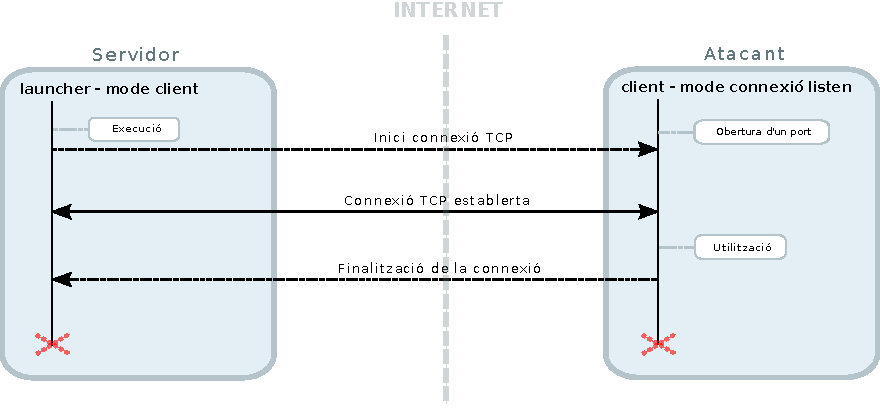
\includegraphics[scale=1,keepaspectratio]{diagrames/solutionDesignClientMode.pdf} \\
    \caption{Esquema del mode client}
    \label{fig:modeClient}
\end{figure}

En la figura podem veureu representada el què seria la màquina de l'atacant (el què utilitza la part client del rootkit),
i la màquina servidor (la ``victima'' que és on s'executa el launcher).

El funcionament seria el següent:
\begin{enumerate}
    \item Prèviament al què es veu a la figura, s'ha de col·locar el launcher en la màquina servidor.
    \item S'executa el client en mode LISTEN a la màquina de l'atacant.
    \item S'executa el launcher en el servidor tot passant per paràmetre l'adreça ip de la màquina i el port on està escoltat
        el client.
    \item El launcher inicia una connexió cap al client.
    \item Un cop establerta, el client pot realitzar l'acció que ha sol·licitat.
    \item Un cop acaba de fer-ne ús, aquest tanca la connexió, i amb aquest acaba el procés launcher en el servidor.
\end{enumerate}

\subsubsection{TCP}
La idea d'aquest mode de comunicació, és la de tenir un servei que permeti executar 
El fet de disposar d'un servei en constant execució o no, és la principal diferència entre el mode servidor
no privilegiat, i el mode client. En aquest mode, tindrem el launcher escoltant a un port TCP esperant que
el client es connecti per a sol·licitar una acció. \\

Aquest mode té l'inconvenient que en un entorn en què tinguem algun firewall, molt probablement, no ens 
servirà de res ja que les connexions cap al port del nostre launcher, molt probablement no estaran permeses. \\

\begin{figure}[htp]
    \centering
    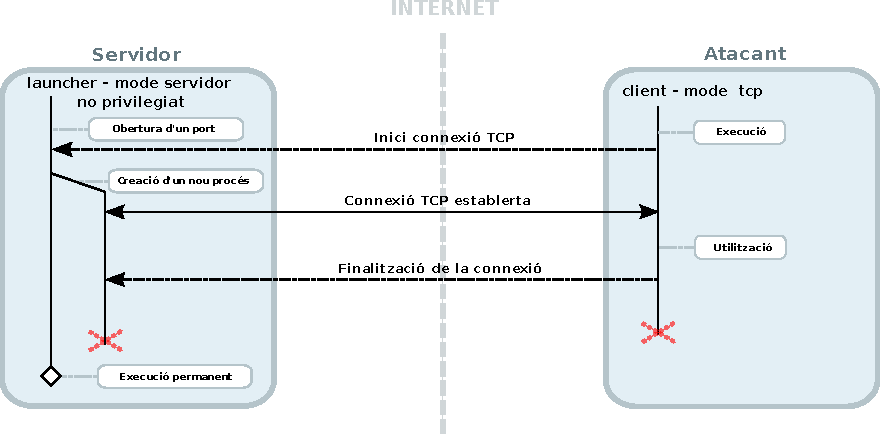
\includegraphics[scale=1,keepaspectratio]{diagrames/solutionDesignUnprivilegedServerMode.pdf} \\
    \caption{Esquema del mode servidor no privilegiat}
    \label{fig:modeUnprivilegedServer}
\end{figure}


Aquest mode de comunicació, és utilitzat només en el cas en què el client vulgui connectar-se a un launcher que
s'ha executat en mode servidor no privilegiat. \\

El protocol de comunicació (figura \ref{fig:modeUnprivilegedServer}) en aquest cas és: \\

\begin{enumerate}
    \item El client estableix una connexió TCP amb a la màquina i port on està escoltant el launcher
    \item El client envia un paquet autenticat cap al launcher, especificant-li l'acció a portar a terme
    \item El launcher efectua l'acció, utilitzant la mateixa connexió ja establerta per a comunicar-se
\end{enumerate}

\subsection{Mode privilegiat}

A diferència del mode no privilegiat, aquest cop els dos modes de comunicació poden ser utilitzats sense cap requeriment de com
el launcher és executat. \\


El mode servidor privilegiat, és el mode que requereix de permisos d'administrador, i que alhora ens permetrà
fer ús de les característiques mes avançades del rootkit. \\

La principal diferència entre aquest mode de funcionament, és que al disposar de permisos d'administrador a
la màquina, podem realitzar tasques molt més avançades. Entre elles, tenim la possibilitat d'implementar 
sniffers a nivell d'aplicació per tal de poder capturar passwords, o el fet de poder utilitzar RAW sockets que
ens permetran utilitzar diferents modes de comunicació (se'n comenta el disseny més endavant), per tal de 
saltar-se la majoria de configuracions de firewall. \\

Per tots aquests motius, sempre que sigui possible ens interessarà utilitzar el rootkit en aquest mode. \\

El funcionament del rootkit quan s'està executant en mode privilegiat, varia depenent el tipus de connexió
que prefereix realitzar el client en aquell moment. Més endavant quan s'expliquen els modes de comunicació disponibles
en aquest mode (figures \ref{fig:modePrivilegedServerREV} i \ref{fig:modePrivilegedServerREV}), es detalla el seu funcionament. \\


\subsubsection{REV}

Aquest mode de comunicació, es pot utilitzar només en el cas d'haver llançat el launcher en mode privilegiat.
El nom de REV, prové de la idea principal del mode de comunicació que és l'ús d'una comunicació reversa on 
és el client qui (a través d'un port ja obert en la màquina), sol·licita que el rootkit es connecti cap a ell. \\

El protocol de comunicació és el següent: \\

\begin{figure}[htp]
    \centering
    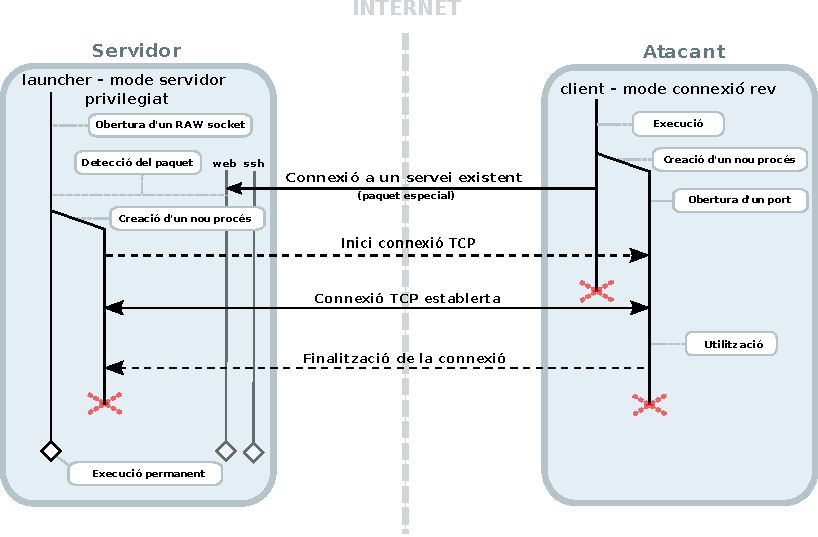
\includegraphics[scale=1,keepaspectratio]{diagrames/solutionDesignPrivilegedServerModeREV.pdf} \\
    \caption{Esquema del mode de connexió revers}
    \label{fig:modePrivilegedServerREV}
\end{figure}

\begin{enumerate}
    \item El client obre un servei que es queda escoltant a un port esperant la connexió del launcher.
    \item El client llança un procés fill que es connecta a un port TCP qualsevol de la màquina on s'està 
        executant el rootkit. Aquest port ha d'haver estat obert per qualsevol altre servei del sistema (per 
        exemple el típic servei web).
    \item El client envia un paquet autenticat través d'aquesta connexió. Aquest paquet serà probablement  
        descartat pel servei al no ser un paquet que compleixi el protocol del servei, però serà detectat per
        part del rootkit.
    \item El rootkit detectarà i comprovarà el paquet, i en cas de ser vàlid, establirà una connexió TCP cap 
        al client.
    \item Un cop establerta la connexió amb el client, s'utilitzarà aquesta per tal d'efectuar l'operació 
        demandada.
\end{enumerate}

Els principals avantatges son: \\

\begin{itemize}
    \item La comunicació entre launcher i client és molt fiable i és provable que sobrepassi la majoria de 
        configuracions de xarxa d'una manera totalment vàlida.
    \item Per executar el client, no necessitem permisos de superusuari.
\end{itemize}

Els principals desavantatges són: \\

\begin{itemize}
    \item El primer és que requerim que la màquina disposi d'alguna aplicació que escolti en algun port 
        TCP. Tot i que això no acostuma a ser difícil, hi han casos en què no és així.
    \item El segon és que un cop el rootkit ha establer la connexió TCP amb el client, aquesta connexió
        apareix en el llistat de connexions establertes de la màquina, i en segons quina màquina, això
        pot ser molt sospitós per a l'administrador.
\end{itemize}

Per tal d'utilitzar aquest mode de comunicació, cal que la màquina on s'executa el client, tingui almenys
un port de la ip pública, assignat a ella, de manera que sigui possible lo comunicació directe des de fora
la xarxa local. En configuracions personals com una línia ADSL amb router, caldria que el router de la màquina
on l'executés el client, tingués un ``port obert'' (un port amb DNAT) per tal que el rootkit es pogués 
connectar a ell. Aquest requisit també existeix en els següents modes de comunicació (RAW i LISTEN). \\

\subsubsection{RAW}

Igual que en el cas anterior, aquest mode de comunicació només pot ser utilitzat en cas d'haver llançat el launcher
en mode privilegiat. \\

Per tal d'implementar aquest mode de comunicació, s'ha hagut d'implementar un protocol de capa de transport 
compatible amb el subset de paquets vàlids pel protocol TCP (documentat més endavant). D'aquesta manera s'ha 
aconseguit poder transmetre per internet paquets TCP vàlids, que a nivell de sessió són aparentment invàlids. 
Com que tots aquests paquets són entregats a la màquina, el nostre rootkit és capaç d'interpretar-los i 
respondre obtenint com a resultat un protocol de comunicació invisible per el nucli del sistema operatiu. \\

Fer tot això, ens aporta principalment dos avantatges: \\

\begin{enumerate}
    \item Que les connexions establertes utilitzant aquest mode, són gairebé invisibles (caldria analitzar els
        diferents paquets de xarxa per detectar una connexió d'aquest tipus)
    \item Que no necessitem tenir cap aplicació escoltant a un port per tal de comunicar-nos amb el launcher.
\end{enumerate}

El nom de mode de comunicació RAW, prové del tipus de socket que ens permet implementar tot això (RAW socket),
i el seu funcionament és el següent: \\

\begin{figure}[htp]
    \centering
    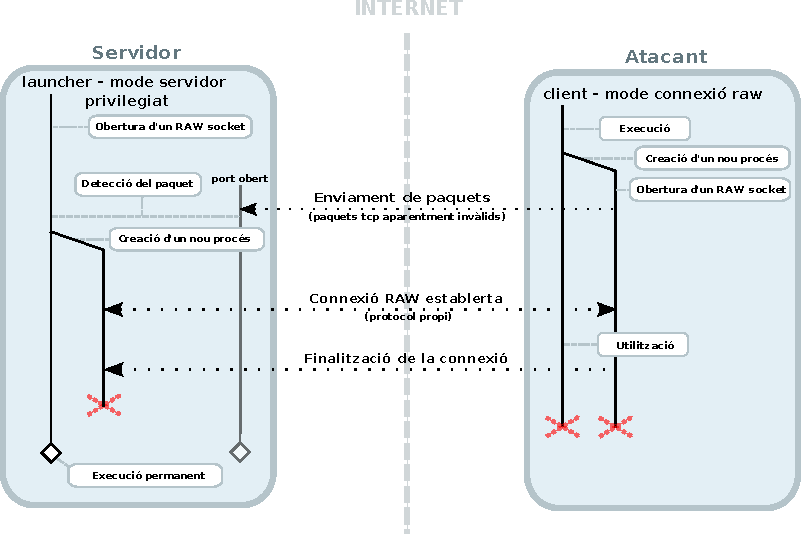
\includegraphics[scale=1,keepaspectratio]{diagrames/solutionDesignPrivilegedServerModeRAW.pdf} \\
    \caption{Esquema del mode de connexió revers}
    \label{fig:modePrivilegedServerRAW}
\end{figure}

\begin{enumerate}
    \item Primer de tot, el client inicialitza un socket RAW per tal de comunicar-se amb el launcher.
    \item El client crea un procés per tal d'enviar envia el paquet d'autenticació a la màquina i port escollits,
        i espera que el launcher li respongui.
    \item Un cop el launcher rep el paquet, comprova si el paquet és d'alguna connexió existent, i si no
        ho és, crea un altre procés destinat als enviaments de paquets cap al client. Alhora, comença a
        processar l'acció que li ha sol·licitat el client, tot utilitzant els paràmetres rebuts per a la 
        comunicació.
    \item En el moment que el client rep una resposta del launcher, comença a processar l'acció tenint
        ja la connexió establerta.
\end{enumerate}

L'objectiu de crear un protocol propi de comunicació, era aconseguir comunicar el client i el launcher per
internet sense que les utilitats del sistema operatiu per visualitzar les connexions de xarxa establertes
s'adonessin de les connexions entre launcher i client. En definitiva, l'objectiu és aconseguir passar més 
desapercebuts. \\

Per tal de poder aconseguir això i establir una comunicació a través d'internet, calia utilitzar un subset de 
paquets IP vàlids per a tota l'electrònica de xarxa que hi ha a internet. Per aquest motiu, es va escollir
utilitzar paquets vàlids del protocol TCP, però que són invàlids ja que fan referència a una sessió inexistent.
A més, per tal de afavorir que els paquets eren entregats, aquests eren enviats amb el flag de RESET activat. 
Aquesta peculiaritat fa que en alguns firewalls de baixa qualitat configurats amb una política de restricció de 
tots els paquets entrants menys els paquets que formen part d'una connexió ja establerta, detectin que el paquet
fa referència a una connexió ja establerta\footnote{Molts d'aquests firewalls, només afegeixen una regla denegant
els paquets amb el flag SYN, ja que només intenten denegar el inici d'una connexió TCP.} i el deixin passar. \\

Cal dir que aquest protocol es podria millorar força tot afegint algoritmes de control i retransmissió. Actualment
el nostre protocol de comunicació RAW, es podria dir que només ofereix les característiques del protocol UDP
\footnote{El protocol UDP és un protocol de transmissió que permet l'enviament de dades sense haver d'iniciar una 
sessió. Les dades enviades utilitzant aquest protocol, no són confirmades per el receptor i per tant la comprobació
s'ha de fer a nivell d'aplicació.}. Més endavant en el capítol solucions, s'explica amb tot detall el seu funcionament. \\

Els paquets transmesos per la xarxa segueixen aquesta estructura: \\

\begin{figure}[htp]
    \centering
    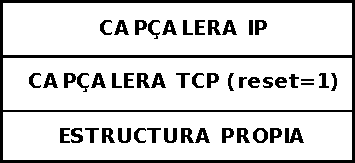
\includegraphics[scale=1,keepaspectratio]{diagrames/solutionDesignPacketStructure.pdf} \\
    \caption{Esquema d'un paquet RAW}
    \label{fig:packetScheme}
\end{figure}

En definitiva són paquets TCP amb el flag RESET activat, i una estructura de dades que detallem a continuació.

\subsection{Paquet de comunicació}

La següent estructura, s'utilitza en dos casos diferenciats:
\begin{itemize}
    \item L'enviament de paquets de control.
    \item L'enviament de paquets d'una connexió RAW.
\end{itemize}

Els paquets de control, són tots aquells que sol·liciten realitzar una acció tant del client al launcher, com a l'inrevés.
Els d'una connexió RAW són els comentats en el punt anterior.

El fet de que el client sol·liciti una acció al launcher, implica l'enviament d'un paquet de control del client sol·licitant
la realització d'una acció. 

\begin{Verbatim}[commandchars=@\[\]]
@PYay[struct] data {
    @PYaJ[unsigned] @PYaJ[char] pass@PYZlb[]@PYag[20]@PYZrb[];
    @PYaJ[unsigned] @PYaJ[char] action;
    @PYaJ[unsigned] @PYaJ[short] port;
    @PYaJ[unsigned] @PYaJ[long] size;
    @PYaJ[unsigned] @PYaJ[char] bytes@PYZlb[]BUFSIZE@PYZrb[];
} __attribute__ ((packed));
\end{Verbatim}

Podem veure que aquesta estructura conté un array de 20 bytes anomenat pass. És en aquest camp on tant el launcher
com el client s'han d'autenticar l'un amb l'altre, és a dir, tant el launcher ha de conèixer el password que ha introduït 
el client, com el client el client ha de conèixer el password amb el què va estar compilat el launcher.\\

Pel què fa als altres paràmetres, ``action'' fa referència a la acció\footnote{Es pot 
veure aquest camp, com el camp que especifica com ha de fer servir el valor dels altres pàmetres.}, ``port'' al port a 
utilitzar, ``size'' al nombre de bytes utiiltzats en el buffer ``bytes''.

